\documentclass[english,compress]{beamer}

\mode<presentation>
{
  \useoutertheme[footline=titleinstituteauthor]{c4}
  \useinnertheme{circles}
  \usecolortheme{whale}
  \usecolortheme{orchid}
  \usecolortheme{c4}
  %\setbeamercovered{transparent}
  \setbeamercovered{highly dynamic}
  \setbeamertemplate{caption}{\insertcaption}
}

\usepackage{babel}
\usepackage[utf8]{luainputenc}
\usepackage{fontspec}

\usepackage{graphicx}
\usepackage{color}
\usepackage{listings}
\usepackage{tikz}
\usetikzlibrary{shapes,arrows,matrix,decorations.pathreplacing}

\definecolor{dark-green}{RGB}{5, 148, 5}
\lstset{
language=C,
basicstyle=\ttfamily,
keywordstyle=\color{blue}\bfseries,
commentstyle=\color{dark-green}\slshape,
stringstyle=\color{purple},
breaklines=true,
breakatwhitespace=true,
prebreak=\raisebox{0ex}[0ex][0ex]{\ensuremath{\hookleftarrow}},
tabsize=2,
numbers=left,
numberstyle=\tiny,
moredelim=[is][\sl]{$}{$},
escapechar=\%,
morekeywords={size_t, _Bool, uint8_t, int8_t, uint16_t, int16_t, uint32_t, int32_t}
}

% Multimedia
%\usepackage{multimedia}

\title{U23 C Workshop}

\author[Florian Zeitz <florob@babelmonkeys.de>]{Florian ``Florob'' Zeitz}

\institute[Chaos Computer Club Cologne]
{
Chaos Computer Club Cologne e.V.\\
http://koeln.ccc.de \\
}

\date{2013-10-19}

\pgfdeclareimage[height=1cm]{barcode}{./c4-logo}
\logo{\pgfuseimage{barcode}}


% Folgendes sollte gelC6scht werden, wenn man nicht am Anfang jedes
% Unterabschnitts die Gliederung nochmal sehen möchte.
\AtBeginSection[]
{
	\begin{frame}<beamer>
		\begin{columns}
		\column{0.5\textwidth}
			\tableofcontents[sections={<1-2>},currentsection,currentsubsection]
		\column{0.5\textwidth}
			\tableofcontents[sections={<3>},currentsection,currentsubsection]
		\end{columns}
	\end{frame}
}

% Falls Aufzählungen immer schrittweise gezeigt werden sollen, kann
% folgendes Kommando benutzt werden:
%\beamerdefaultoverlayspecification{<+->}


\begin{document}

\begin{frame}
  \titlepage
\end{frame}

\begin{frame}{Outline}
	\begin{columns}
	\column{0.5\textwidth}
		\tableofcontents[sections={<1-2>}]
	\column{0.5\textwidth}
		\tableofcontents[sections={<3>}]
	\end{columns}
\end{frame}

\section{History}
\begin{frame}
	\begin{columns}
	\column{0.7\textwidth}
	\begin{itemize}
		\item Initially written in the context of Unix
		\item[1978] ``The C Programming Language'' by Kernighan and Ritchie (first informal specification, K\&R C)
		\item[1983] ANSI forms a committee to standardize C
		\item[1988] ``The C Programming Language'' 2nd Edition, updated to reflect ANSI specification
		\item[1989] Specification approved by the ANSI (ANSI C/C89)
		\item[1990] Identical specification approved by the ISO (C90)
		\item[1999] Updated ISO specification (C99)
		\item[2011] Updated ISO specification (C11)
	\end{itemize}
	\column{0.3\textwidth}
	\begin{figure}[h]
		\begin{center}
			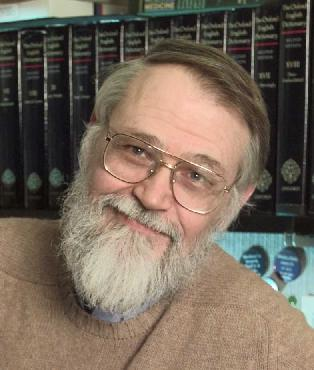
\includegraphics[width=0.5\textwidth]{kernighan.jpg}
		\end{center}
		\caption{Brian Kernighan}
	\end{figure}
	\begin{figure}[h]
		\begin{center}
			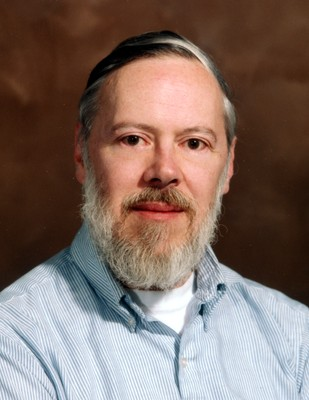
\includegraphics[width=0.5\textwidth]{ritchie.jpg}
		\end{center}
		\caption{Dennis Ritchie}
	\end{figure}
	\end{columns}
\end{frame}

\section{Basics}

\begin{frame}{Compiling code}
  \tikzstyle{file} = [draw, thin, fill=c4lightblue]
  \tikzstyle{proc} = [ellipse, draw, thin, fill=c4orange!90, minimum height=2.5em]
  \begin{figure}
    \begin{tikzpicture}[node distance=2cm, >=stealth', thick]
	    \node[file] (c1) {.c File};
	    \node[file, node distance=1cm, above of=c1] (h1) {.h File};
	    \node[proc, right of=c1] (cpp1) {\texttt{cpp}};
	    \node[proc, right of=cpp1] (comp1) {\texttt{cc}};
	    \node[file, right of=comp1] (o1) {.o File};

	    \node[file, below of=c1] (c2) {.c File};
	    \node[file, node distance=1cm, above of=c2] (h2) {.h File};
	    \node[proc, right of=c2] (cpp2) {\texttt{cpp}};
	    \node[proc, right of=cpp2] (comp2) {\texttt{cc}};
	    \node[file, right of=comp2] (o2) {.o File};

	    \node[file, below of=c2] (c3) {.c File};
	    \node[file, node distance=1cm, above of=c3] (h3) {.h File};
	    \node[proc, right of=c3] (cpp3) {\texttt{cpp}};
	    \node[proc, right of=cpp3] (comp3) {\texttt{cc}};
	    \node[file, right of=comp3] (o3) {.o File};

	    \node[proc, right of=o2] (linker) {\texttt{ld}};

	    \node[file, above of=linker] (a) {.a File};

	    \node[file, right of=linker] (elf) {ELF File};

	    \draw[->] (c1) -- (cpp1);
	    \draw[->] (h1) -- (cpp1);
	    \draw[dotted,<-] (c1) -- (h1);
	    \draw[->] (cpp1) -- (comp1);
	    \draw[->] (comp1) -- (o1);
	    \draw[->] (c2) -- (cpp2);
	    \draw[->] (h2) -- (cpp2);
	    \draw[->] (h3) -- (cpp2);
	    \draw[dotted, <-] (c2) -- (h2);
	    \draw[dotted, <-] (c2) -- (h3);
	    \draw[->] (cpp2) -- (comp2);
	    \draw[->] (comp2) -- (o2);
	    \draw[->] (c3) -- (cpp3);
	    \draw[->] (cpp3) -- (comp3);
	    \draw[->] (comp3) -- (o3);
	    \draw[->] (o1) -- (linker);
	    \draw[->] (o2) -- (linker);
	    \draw[->] (o3) -- (linker);
	    \draw[->] (a) -- (linker);
	    \draw[->] (linker) -- (elf);
    \end{tikzpicture}
  \end{figure}
\end{frame}

\subsection{Hello World}
\begin{frame}[fragile]{Hello World}
	\begin{lstlisting}
		#include <stdio.h> %\visible<2->{$\leftarrow$ \parbox{0.5\textwidth}{\it Include definitions for standard IO}}%

		int main(void) %\visible<3->{$\leftarrow$ \parbox{0.4\textwidth}{\it Entry point}}%
		{
		  printf("Hello World\n"); %\visible<4->{$\leftarrow$ \parbox{0.35\textwidth}{\flushleft\it Write: Hello World<newline>}}%

		  return 0; %\visible<5->{$\leftarrow$ \parbox{0.45\textwidth}{\flushleft\it Return success (0) to the system}}%
		}
	\end{lstlisting}
\end{frame}

\begin{frame}[fragile]{Expressions}
	\begin{itemize}
		\item $\underbrace{\overbrace{\text{\lstinline|printf("Hello World\n")|}}^{\text{Expression}}\text{\lstinline|;|}}_{Statement}$
		\item  ``An expression is a sequence of operators
			and operands that specifies computation of a value,
			or that designates an object or a function,
			or that generates side effects, or that
			performs a combination thereof.''
		\item Almost everything is an expression
		\item An expression followed by a \lstinline|;| is a statement
	\end{itemize}

\end{frame}

\begin{frame}[fragile]{Blocks}
	\begin{lstlisting}
		#include <stdio.h>

		int main(void)
		{ %\begin{tikzpicture}[overlay] \draw[decorate,decoration={brace,amplitude=5pt},thick] (6,0.1) -- +(0,-2) node[midway,right,xshift=4pt] {\it Block};\end{tikzpicture}%
		  printf("Hello World\n");

		  return 0;
		}
	\end{lstlisting}
	\begin{itemize}
		\item Also known as \textit{compound statements}
		\item Collection of statements, often can be used in place of a single statement
		\item Relevant for scope (we'll talk about this later)
	\end{itemize}
\end{frame}

\subsection{Variables}
\begin{frame}{Type system}
	\begin{itemize}
		\item C is statically typed
		\item Variables require a declaration, including type
		\item {\color{blue}\lstinline|$type$|} \lstinline|var;|
		\item Variables can be declared as \lstinline|const| meaning
			their value can only be initialized, but never changed
	\end{itemize}
\end{frame}

\begin{frame}{Integer types}
	\begin{table}
		\centering
		\begin{tabular}{l|l|l}
			Name & Domain & Constant \\
			\hline
			\lstinline|_Bool| & \{0, 1\} & \lstinline|0| \\
			\lstinline|char| & [$-2^7$, $2^7-1$] & \lstinline|5| or \lstinline|'a'| \\
			\lstinline|int| & [\lstinline|INT_MIN|, \lstinline|INT_MAX|] & \lstinline|5| \\
			\lstinline|unsigned int| & [0, \lstinline|UINT_MAX|] & \lstinline|5u| \\
			{\color{blue}\bf\lstinline|int$X$_t|} & [$-2^{X-1}$, $2^{(X-1)}-1$] $ X \in \{8, 16, 32\}$ & \lstinline|6| \\
			{\color{blue}\bf\lstinline|uint$X$_t|} & [0, $2^X-1$] $ X \in \{8, 16, 32\}$ & \lstinline|6u|
		\end{tabular}
	\end{table}
\end{frame}

\begin{frame}{Floating-point types}
	\begin{table}
		\centering
		\begin{tabular}{l|l|p{0.35\textwidth}}
			Name & Domain & Constant \\
			\hline
			\lstinline|float| & $\subset \mathbb{R}$ & \lstinline|1.5f| or \lstinline|.3f| or \lstinline|4.f| or \lstinline|5e3f| or \lstinline|0x4a.b2p4f| \\
			\lstinline|double| & $\subset \mathbb{R}$ (more values than \lstinline|float|) & \lstinline|1.5| or \lstinline|.3| or \lstinline|4.| or \lstinline|5e3| or \lstinline|0x4a.b2p4|
		\end{tabular}
	\end{table}
\end{frame}

\begin{frame}{Void}
	\begin{itemize}
		\item signals the absence of data (its domain is empty)
		\item \lstinline|void| is an incomplete type
		\item[$\Rightarrow$] no variable of type \lstinline|void|
			can be declared
	\end{itemize}
\end{frame}

\begin{frame}{Casts}
	\begin{itemize}
		\item types can be converted to each other
		\item converting the value of an expression to another type is called cast
		\item this can be done explicitly by prefixing the expression by a type in parentheses
		\item e.\,g.\ \lstinline|(uint8_t)1025| (effectively a modulo 256)
	\end{itemize}
\end{frame}

\begin{frame}{Scope}
	\begin{itemize}
		\item region of program text where a variable is visible
		\item C uses file and block scope
		\item variables declared outside a block have file scope,
			others have block scope
	\end{itemize}
\end{frame}

\begin{frame}[fragile]{Scope}
	\begin{lstlisting}
		void f(void)
		{ %\begin{tikzpicture}[overlay] \draw[decorate,decoration={brace,amplitude=5pt},thick] (4.7,0.1) -- +(0,-3.5) node[midway,right,xshift=4pt] {\it Scope/Lifetime of {\sf a}};\end{tikzpicture}%
		  int a;

		  { %\begin{tikzpicture}[overlay] \draw[decorate,decoration={brace,amplitude=5pt},thick] (1.7,0.1) -- +(0,-1) node[midway,right,xshift=4pt] {\parbox{2cm}{\it Scope/Lifetime of {\sf b}}};\end{tikzpicture}%
		    int b;
		  }

		}
	\end{lstlisting}
\end{frame}

\begin{frame}{Storage classes}
	\begin{itemize}
		\item how variables are stored can be modified
		\item \lstinline|auto|: lifetime is the associated block (default, rarely used explicitly)
		\item \lstinline|static|: lifetime is the entire program execution
		\item \lstinline|extern|: the variable belongs to another module
		\item \lstinline|register|: access should be as fast as possible (in a register), can be ignored
	\end{itemize}
\end{frame}

\begin{frame}[fragile]{printf()}
	\begin{lstlisting}[numbers=none]
		int printf(const char *fmt, ...);
	\end{lstlisting}
	\begin{itemize}
		\item takes a format string and any number of other parameters
		\item prints a string to stdout with the parameter formatted according to the format string
		\item[\%i, \%d] prints an \lstinline|int| (anything smaller than  \lstinline|int| is automatically converted to one here)
		\item[\%f] prints a \lstinline|double| (\lstinline|float|s are automatically converted to \lstinline|double| here)
		\item[\%s] prints a \lstinline|char*| (string)
		\item[\%c] prints an \lstinline|int| as ASCII character
	\end{itemize}
\end{frame}

\begin{frame}{Escape sequences}
	\begin{itemize}
		\item[\textbackslash n] new line
		\item[\textbackslash r] carriage return
		\item[\textbackslash t] horizontal tab
		\item[\textbackslash\textbackslash] backslash
		\item[\textbackslash '] single quote
		\item[\textbackslash "] double quote
		\item[\textbackslash \textit{<oct>}] ASCII character \textit{<oct>}
		\item[\textbackslash x\textit{<hex>}] ASCII character \textit{<hex>}
	\end{itemize}
\end{frame}

\begin{frame}[fragile]{printf()}
	\begin{lstlisting}[escapechar=]
		int main(void) {
		  printf("%c: %i\n", 'a', 8);

		  return 0;
		}
	\end{lstlisting}
	Output: \verb|a: 8|
\end{frame}

\subsection{Logical Operations}
\begin{frame}{Boolean values}
	\begin{itemize}
		\item Everything that is not equal to 0 is interpreted as true
		\item Everything equal to 0 is false
		\item Logical operations always evaluate to 0 or 1
	\end{itemize}
\end{frame}

\begin{frame}{Negation, Relational/Equality Operators}
	\begin{itemize}
		\item \lstinline|!a|: negation
		\item \lstinline|a < b|: less than
		\item \lstinline|a > b|: greater than
		\item \lstinline|a <= b|: less than or equal
		\item \lstinline|a >= b|: greater than or equal
		\item \lstinline|a == b|: equal
		\item \lstinline|a != b|: not equal
	\end{itemize}
\end{frame}

\begin{frame}{Logical AND/OR}
	\begin{itemize}
		\item \lstinline|$exp1$ && $exp2$|: logical and (if \textit{exp1} is false, \textit{exp2} is not evaluated
		\item \lstinline@$exp1$ || $exp2$@: logical or (if \textit{exp1} is true, \textit{exp2} is not evaluated)
		\item left-to-right evaluation is guaranteed, side-effects
			of \textit{exp2} might not take place
	\end{itemize}
\end{frame}

\subsection{Arithmetic Operations}
\begin{frame}{Arithmetic Operators}
	\begin{itemize}
		\item \lstinline|a + b|: Addition
		\item \lstinline|a - b|: Subtraction
		\item \lstinline|a * b|: Multiplication
		\item \lstinline|a / b|: Division
		\item \lstinline|a \% b|: Modulo
	\end{itemize}
\end{frame}

\begin{frame}{Short forms}
	\begin{itemize}
		\item \lstinline|a += 3|: Same as \lstinline|a = a + 3|
		\item \lstinline|a -= 3|: Same as \lstinline|a = a - 3|
		\item \lstinline|a *= 3|: Same as \lstinline|a = a * 3|
		\item \lstinline|a /= 3|: Same as \lstinline|a = a / 3|
		\item \lstinline|a \%= 3|: Same as \lstinline|a = a \% 3|
		\item \lstinline|a++|: (Post-)Increment, evaluates to a's old value
		\item \lstinline|a--|: (Post-)Decrement, evaluates to a's old value
		\item \lstinline|++a|: (Pre-)Increment, evaluates to a's new value
		\item \lstinline|--a|: (Pre-)Decrement, evaluates to a's new value
	\end{itemize}
\end{frame}

\subsection{Loops}
\begin{frame}[fragile]
	\begin{block}{while-Loop}
		\begin{lstlisting}[numbers=none]
			while($condition$) $statement/block$
		\end{lstlisting}
		\begin{itemize}
			\item Runs as long as \textit{condition} is true
			\item \textit{condition} is evaluated \emph{before} each iteration
		\end{itemize}
	\end{block}
	\begin{block}{do-while-Loop}
		\begin{lstlisting}[numbers=none]
			do $statement/block$ while($condition$)
		\end{lstlisting}
		\begin{itemize}
			\item Runs as long as \textit{condition} is true
			\item \textit{condition} is evaluated \emph{after} each iteration
			\item[$\Rightarrow$] runs at least once
		\end{itemize}
	\end{block}
\end{frame}

\begin{frame}[fragile]
	\begin{block}{for-Loop}
		\begin{lstlisting}[numbers=none]
			for($initialization$; $condition$; $expression$)
			  $statement/block$
		\end{lstlisting}
		\begin{itemize}
			\item Executes \textit{initialization}
			\item Runs as long as \textit{condition} is true
			\item \textit{condition} is evaluated before each iteration
			\item Executes \textit{Expression} after each iteration
		\end{itemize}
	\end{block}
\end{frame}

\begin{frame}[fragile]{Example: Print the alphabet}
	\begin{lstlisting}
		for (char c = 'a'; c <= 'z'; c = c+1)
		  putchar(c);
	\end{lstlisting}
\end{frame}

\begin{frame}{Changing the flow}
	\begin{itemize}
		\item \lstinline|continue|: Jumps imediately to the next loop iteration (checking the condition first)
		\item \lstinline|break|: Terminates the loop prematurely
	\end{itemize}
\end{frame}

\subsection{Branches}
\begin{frame}[fragile]
	\begin{block}{if-Statement}
		\begin{lstlisting}[numbers=none]
			if($condition$) $statement/block$
			if($condition$) $statement/block$ else $statement/block$
		\end{lstlisting}
		\begin{itemize}
			\item if \textit{condition} is true execute the first statement
			\item if \textit{condition} is false execute the second statement

		\end{itemize}
	\end{block}
\end{frame}

\begin{frame}[fragile]
	\begin{block}{switch-Statement}
		\begin{lstlisting}[numbers=none]
			switch($condition$) $statement/block$
		\end{lstlisting}
		\begin{itemize}
			\item jumps to a statement labeled ``\lstinline|case $condition$|'' within the switch body
			\item if no such label exists jumps to a statement labeled ``\lstinline|default|''
			\item if no such label exists jumps past the switch body
			\item switch body can be left with \lstinline|break|
		\end{itemize}
	\end{block}
\end{frame}

\begin{frame}[fragile]{Example: Fibonacci}
	\begin{lstlisting}
		int fib(int i)
		{
		  switch(i) {
		  case 0:
		  case 1:
		    return i;
		  default:
		    return fib(i-1) + fib(i-2);
		  }
		}
	\end{lstlisting}
\end{frame}

\begin{frame}[fragile]{Example: Print a number}
	\begin{lstlisting}
		void printNumber(int num)
		{
		  switch (num) {
		  case 0:
		    puts("Zero");
		    break;
		  case 1:
		    puts("One");
		    break;
		  default:
		    puts("Computers only use zeros and ones");
		  }
		}
	\end{lstlisting}
\end{frame}

\begin{frame}[fragile]{Exercises 1}
	\begin{center}
		Compiling code: \verb|gcc -std=c99 -Wall -o output input.c|
	\end{center}
	\begin{enumerate}
		\item Write, compile and execute a Hello World program
		\item Write a program that prints the faculty of the numbers 0 to 10 using an iterative approach
		\item Write a program that prints the first 10 fibonacci numbers using an iterative approach
		\item Write a program that prints all primes between 2 and 100
		\item Write a program that calculates the 5th power of all numbers from 2 to 10
	\end{enumerate}
\end{frame}

\subsection{Functions}
\begin{frame}{Functions}
	\begin{itemize}
		\item each function has a declaration and a definition
		\item declarations are usually provided in separate header files
		\item declaration: ``This function exists and returns {\color{blue}\lstinline|$type$|}''
		\item definition: ``This function works as follows''
	\end{itemize}
\end{frame}

\begin{frame}[fragile]{Declaration and Prototype}
	\begin{lstlisting}[numbers=none]
		%{\it\color{blue}type1}% func(%{\it\color{blue}{type2}% param1);
	\end{lstlisting}
	\begin{itemize}
		\item declares a function returning {\color{blue}\lstinline|$type1$|}, with one parameter of type {\color{blue}\lstinline|$type2$|}
		\item is both a declaration and a prototype
		\item prototype: ``This function's parameters have this types''
		\item parameter names may be omitted
		\item a function without parameters is declared with \lstinline|void| as parameter list
	\end{itemize}
\end{frame}

\begin{frame}[fragile]{Definition}
	\begin{lstlisting}[numbers=none]
		%{\it\color{blue}type1}% func(%{\it\color{blue}{type2}% param1)
		  $block$
	\end{lstlisting}
	\begin{itemize}
		\item defines a function
		\item must match the prototype
		\item can double as declaration/prototype
	\end{itemize}
\end{frame}

\begin{frame}[fragile]{Exercises 2}
	\begin{enumerate}
		\item Write a program that prints the faculty of the numbers 0 to 10 using a recursive approach
		\item Write a program that prints the first 10 fibonacci numbers using a recursive approach
		\item Implement a function that calculates the area of a triangle and test it
		\item Implement a function returning the distance between two 3d points (6 double parameters) using \lstinline|double sqrt(double x);| from \lstinline|<math.h>|, add \verb|-lm| to the compile command
		\item Implement a program that counts the number of \lstinline|'l'|s in the input using \lstinline|int getchar(void);|
	\end{enumerate}
\end{frame}

\section{Advanced}
\subsection{Bit Operations}
\begin{frame}{Bit Operations}
	\begin{itemize}
		\item \lstinline|a << b|: Shift \lstinline|a| left by \lstinline|b| Bit
		\item \lstinline|a >> b|: Shift \lstinline|a| right by \lstinline|b| Bit
		\item \lstinline|a & b|: Bitwise and
		\item \lstinline@a | b@: Bitwise or
		\item \lstinline|a ^ b|: Bitwise exclusive or
		\item These support the same short form as the arithmetic operations, e.\,g.\ \lstinline|a ^= b|
	\end{itemize}
\end{frame}

\subsection{Pointer}
\begin{frame}{Pointer type}
	\begin{itemize}
		\item another scalar type
		\item points to another variable
		\item responsible for a lot of C's power
		\item also responsible for a lot of beginner confusion
	\end{itemize}
\end{frame}

\begin{frame}[fragile]{Pointer type}
	\begin{itemize}
		\item declared as {\it\color{blue}type} \lstinline|*var|
		\item read ``pointer to {\it\color{blue}type}''
		\item contains the address at which a variable is stored
		\item special value \lstinline|NULL| to indicate that
			the pointer is not currently pointing anywhere
	\end{itemize}
\end{frame}

\begin{frame}[fragile]{Address operator}
	\begin{lstlisting}
		int a;
		int *a_p = &a;
	\end{lstlisting}
	\begin{itemize}
		\item The \lstinline|&| operator is used to get the address of a variable
		\item if \lstinline|var| has the type {\it\color{blue}type}
			\lstinline|&var| has the type {\it\color{blue}type*}
		\item above \lstinline|a_p| is said to point to \lstinline|a|
	\end{itemize}
\end{frame}

\begin{frame}[fragile]{Indirection operator}
	\begin{lstlisting}
		int a;
		int *a_p = &a;

		*a_p = 5;
	\end{lstlisting}
	\begin{itemize}
		\item The \lstinline|*| operator is used to get the object stored at an address
		\item if \lstinline|var| has the type {\it\color{blue}type*}
			\lstinline|*var| has the type {\it\color{blue}type}
		\item above \lstinline|*a_p = 5| sets the value of \lstinline|a| to 5
	\end{itemize}
\end{frame}

\begin{frame}[fragile]{\lstinline|sizeof| operator}
	\begin{lstlisting}
		_Bool b;

		if (sizeof(b) > sizeof(char))
		  printf("Booleans are rather large here\n");
	\end{lstlisting}
	\begin{itemize}
		\item The \lstinline|sizeof| operator determines the size of a variable or type
		\item The granularity is the length of a char (one byte)
	\end{itemize}
\end{frame}

\begin{frame}[fragile]{Pointer arithmetic}
	\begin{lstlisting}
		int32_t a;
		int32_t *a_p = &a;

		a_p++;
	\end{lstlisting}
	\begin{itemize}
		\item pointers store plain numbers (addresses)
		\item arithmetic works differently however
		\item addition and subtraction acts in the granularity
			of \lstinline|sizeof(a)|
		\item E.\,g.\ \lstinline|a_p++| above increments the value
			of \lstinline|a_p| by 4
	\end{itemize}
\end{frame}

\subsection{Arrays}
\begin{frame}[fragile]{Arrays}
	\begin{lstlisting}
		int A[4];
	\end{lstlisting}
	\begin{itemize}
		\item aggregate data type
		\item contains a list of multiple adjacent variables
		\item \lstinline|int A[4];| declares an array of 4 integers
		\item indexes start at 0
	\end{itemize}
\end{frame}

\begin{frame}[fragile]{Accessing array members}
	\begin{lstlisting}
		int A[4];

		*(A+2) = 3;
		A[3] = 4;
	\end{lstlisting}
	\begin{itemize}
		\item the expression \lstinline|A| evaluates to a \lstinline|int*| to the first element of \lstinline|A|
		\item elements can therefore be accessed using pointer arithmetic
		\item e.\,g.\ \lstinline|*(A+2) = 3| sets the 3rd element of \lstinline|A| to 3
		\item \lstinline|A[3]| is syntactic sugar for \lstinline|(*((A)+(3)))|
		\item \lstinline|3[A]| is therefore valid, but unintuitive
	\end{itemize}
\end{frame}

\subsection{Structs}
\begin{frame}[fragile]{Structs}
	\begin{columns}
	\column{0.45\linewidth}
	\begin{lstlisting}
		struct $tag$ {
		  int i;
		  char c;
		};
		struct $tag$ s;
		struct $tag$ *s_p = &s;

		s.i = 5;
		s_p->c = 'a';
	\end{lstlisting}
	\column{0.55\linewidth}
	\begin{itemize}
		\item aggregate data type
		\item structured, composed of multiple variables of different types
		\item defined structures are referenced using a tag
		\item members are accessed using \lstinline|.|
		\item \lstinline|s_p->i| exists as syntactic sugar for
			\lstinline|(*s_p).i|
	\end{itemize}
	\end{columns}
\end{frame}

\subsection{Initializers}
\begin{frame}[fragile]{Initializers}
	\begin{lstlisting}
		struct $tag$ s = { 4, 'b' };
		int A[4] = { 1, 2, 3, 4 };
		struct $tag$ t = { .c = 'd', .i = 4 };
		int B[4] = { [2] = 3 };
		char C[] = "Hello";
	\end{lstlisting}
	\begin{itemize}
		\item aggregated types can be initialized using initializers
		\item if not otherwise specified members are initialized in order
		\item a designator can be given to address a specific member
		\item unnamed members are initialized to 0
		\item string literals can also be used as initializers
		\item array length can automatically be determined
	\end{itemize}
\end{frame}

\subsection{Enums}
\begin{frame}[fragile]{Enums}
	\begin{lstlisting}
		enum $tag$ {
		  NAME1, NAME2
		};
		enum month {
		  JAN = 1, FEB, MAR, APR, MAY, JUN,
		  JUL, AUG, SEP, OCT, NOV, DEZ
		};
		enum month birth_month;
	\end{lstlisting}
	\begin{itemize}
		\item integer type with limited number of values
		\item other values can be assigned (acts like a normal integer)
		\item names are declared as integer constants, values
			starting at 0
		\item values can explicitly be assigned to a name
	\end{itemize}
\end{frame}

\subsection{Compound Literals}
\begin{frame}[fragile]{Compound Literals}
	\begin{lstlisting}
		struct $tag$ s_p = &(struct $tag$){ 4, 5 };
	\end{lstlisting}
	\begin{itemize}
		\item syntactically looks like casting a initializer
		\item defines an anonymous object
		\item scope and lifetime as if defined as a variable
	\end{itemize}
\end{frame}


\begin{frame}[fragile]{Exercises 3}
	\begin{lstlisting}[numbers=none]
		char *fgets(char *s, int size, FILE *stream);
		int atoi(const char *nptr); // From <stdlib.h>
	\end{lstlisting}
	\begin{enumerate}
		\item Write a program that counts the number of 1 Bits in an integer read from stdin.
		\item Write a function that exchanges the content of two integer variables
		\item Write a function that sorts an integer array (nothing too fancy $\mathcal O(n^2)$ is fine)
	\end{enumerate}
\end{frame}
\end{document}
